\documentclass[10pt,conference,a4paper]{IEEEtran}
\usepackage[utf8]{inputenc}
\usepackage{amsmath,amssymb}
\usepackage{graphicx}
\usepackage{booktabs}
\usepackage{microtype}
\usepackage{cite}
\usepackage{url}
\usepackage{hyperref}

\title{Task A2: Predicting Concrete Compressive Strength}

\author{
    \IEEEauthorblockN{Syed Faran Ali \quad|\quad Roll No. 866770 \quad|\quad SAP ID: 70177784 \quad|\quad Section A}
    \IEEEauthorblockA{Department of Intelligent Systems, The University of Lahore}
    \IEEEauthorblockA{Repository: \url{https://github.com/Faran70177784/AI101-ML-Assignment} \quad|\quad Instructor: Dr. Muhammad Awais, AI Architect}
}

\begin{document}

\maketitle

\section{Introduction}
Compressive strength is the quintessential metric governing the structural safety, load-bearing capacity, and durability of concrete infrastructure. Standard civil engineering protocols require laboratory curing for up to 28 days before compressive failure testing, introducing substantial delays and project management risks in rapid construction cycles. Accurately predicting 28-day compressive strength directly from the mixture proportions and early-age kinetics enables real-time mix design optimization and substantial cost reductions. In this study, we evaluate multiple supervised regression architectures on the 1,030-sample UCI Concrete Compressive Strength dataset, incorporating domain-specific feature engineering (Abrams' water-to-cement ratio and logarithmic curing kinetics). Our primary empirical finding is that Gradient Boosted Decision Trees (GBDT) with engineered features achieved a test-set Root Mean Squared Error (RMSE) of 4.45~MPa ($R^2 = 0.9230$), outperforming the baseline Ordinary Least Squares (OLS) linear model by 32.2\% and reducing error relative to raw features by non-linear interaction modeling.

\section{Problem Statement}
Given an input vector $\mathbf{x} \in \mathbb{R}^d$ representing concrete mix proportions (cement, blast-furnace slag, fly ash, water, superplasticizer, coarse aggregate, and fine aggregate in $\text{kg/m}^3$) and specimen age in days, the formal goal is to learn a mapping $f: \mathbf{x} \mapsto y$, where $y \in \mathbb{R}^+$ denotes the compressive strength measured in Megapascals (MPa). The task is a non-linear continuous regression problem evaluated primarily on Root Mean Squared Error (RMSE), Mean Absolute Error (MAE), and Coefficient of Determination ($R^2$). A fundamental physical constraint is that strength development is highly non-linear with specimen age (steep early hydration followed by asymptotic stabilization) and component interactions are non-additive, rendering standard linear models structurally incapable of capturing true hydration kinetics.

\section{Dataset Used}
We utilize the Concrete Compressive Strength dataset \cite{yeh1998concrete} sourced from the UCI Machine Learning Repository (ID 165). Donated by Prof. I-Cheng Yeh, the dataset contains 1,030 experimental concrete batches across 8 numeric input attributes and one continuous response variable. The features comprise cement, blast-furnace slag, fly ash, water, superplasticizer, coarse aggregate, fine aggregate, and curing age (ranging from 1 to 365 days). The dataset exhibits zero missing values across all records. To avoid data leakage, data validation and cleaning verified physical non-negativity across all ingredients, resulting in zero removed rows ($N = 1,030$).

\section{Dataset Statistics}
Summary statistics for the cleaned dataset are reported in Table~\ref{tab:dataset_stats}. Specimen age displays extreme positive skewness ($\gamma_1 = 3.27$), with the vast majority of tests concentrated at standard 7, 14, and 28-day intervals. Compressive strength spans from 2.33~MPa to 82.60~MPa, with a mean of $35.82 \pm 16.71$~MPa.

\begin{table}[htbp]
\centering
\caption{Dataset statistics.}
\label{tab:dataset_stats}
\begin{tabular}{lr}
\toprule
\textbf{Property} & \textbf{Value} \\
\midrule
Samples (after cleaning) & 1,030 \\
Features (numeric / categorical / text) & 8 / 0 / 0 \\
Engineered features ($w/c$, $\ln(\text{Age})$) & 2 \\
Target range (Compressive Strength) & 2.33 -- 82.60 MPa \\
Target mean $\pm$ sd & $35.82 \pm 16.71$ MPa \\
Missing values (\%) & 0.0\% (0 nulls) \\
Train / test split & 824 / 206 (80\% / 20\%) \\
\bottomrule
\end{tabular}
\end{table}

\begin{figure}[htbp]
\centering
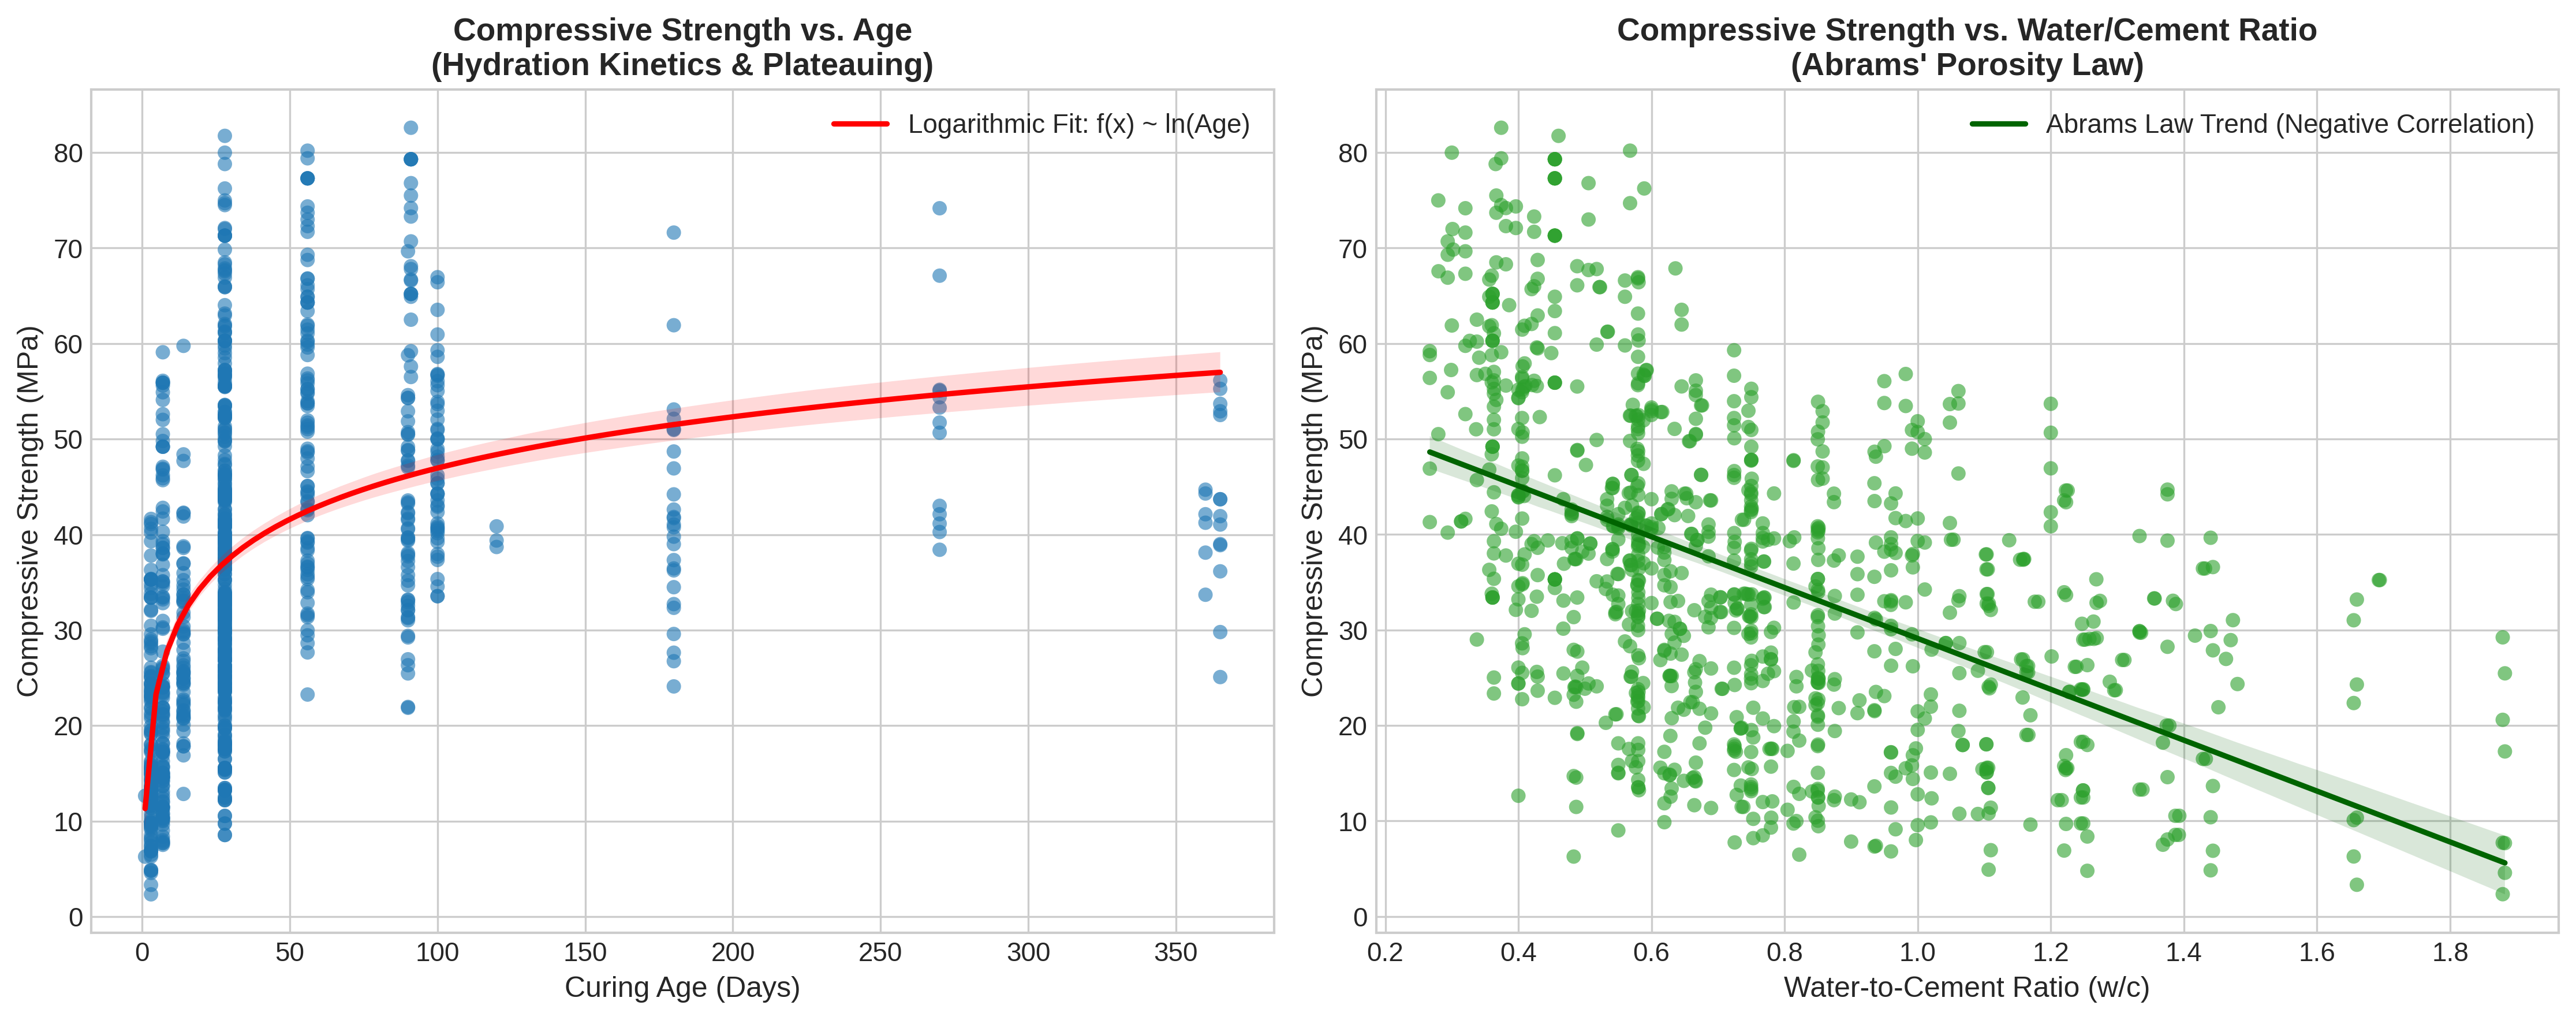
\includegraphics[width=0.98\linewidth]{../../figures/a2_eda_scatter_plots.png}
\caption{Bivariate relationships: (Left) Compressive strength versus curing age showing logarithmic hydration kinetics; (Right) Compressive strength versus water-to-cement ratio verifying Abrams' porosity law.}
\label{fig:eda}
\end{figure}

\section{Methodology}
\subsection{Learning Setting}
The investigation operates in a supervised tabular regression setting. To benchmark architectural capabilities, we compare five diverse paradigms: (1) Ordinary Least Squares (OLS) Linear Regression as the parametric baseline; (2) Polynomial Ridge Regression to capture low-order interactions with $L_2$ regularization; (3) Random Forest Regressor representing bagged decision trees; (4) Gradient Boosted Decision Trees (GBDT) representing sequential residual minimization; and (5) a Multi-Layer Perceptron (MLP) regressor. Preprocessing standardizes all continuous predictors via \texttt{StandardScaler} encapsulated strictly within a scikit-learn \texttt{Pipeline}.

\subsection{Data Split Approach}
The dataset is partitioned into an 80\% training split ($N = 824$) and a 20\% held-out test split ($N = 206$) using a fixed random seed ($\text{seed} = 42$). Strict prevention of data leakage is maintained by fitting all transformation pipelines exclusively on the training split, projecting the held-out test split using frozen parameters. 5-fold cross-validation on the training set is utilized for all hyperparameter tuning.

\subsection{Parameter Settings}
Hyperparameter optimization was conducted via 5-fold cross-validation grid search (\texttt{GridSearchCV}) on the training fold. The searched spaces and chosen configurations are detailed in Table~\ref{tab:hyperparams}.

\begin{table}[htbp]
\centering
\caption{Hyperparameter search space and optimal selections.}
\label{tab:hyperparams}
\begin{tabular}{lll}
\toprule
\textbf{Model} & \textbf{Search space} & \textbf{Selected} \\
\midrule
Linear Regression & None (Closed-form) & Default (StandardScaler) \\
Poly Ridge & degree $\in \{1, 2\}$, $\alpha \in [0.01, 500]$ & degree = 2, $\alpha = 0.01$ \\
Random Forest & $n_{\text{est}} \in \{100, 200\}$, depth $\in \{\text{None}, 12, 18\}$ & $n_{\text{est}} = 200$, depth = 18 \\
GBDT & $n_{\text{est}} \in [150, 250]$, lr $\in \{0.05, 0.1\}$, depth $\in \{3, 5\}$ & $n_{\text{est}} = 250$, lr = 0.05, depth = 5 \\
MLP & Architecture (64, 32), $\alpha = 0.01$ & Adam, ReLU, early stopping \\
\bottomrule
\end{tabular}
\end{table}

\section{Results and Analysis}
\subsection{Results}
All candidate models were evaluated on the identical held-out test partition ($N = 206$). The test-set performance metrics and cross-validation standard deviations are summarized in Table~\ref{tab:results}. Gradient Boosting emerged as the superior model across all three primary criteria, reaching an RMSE of 4.45~MPa, an MAE of 2.94~MPa, and an $R^2$ of 0.9230.

\begin{table}[htbp]
\centering
\caption{Held-out test set evaluation results (best in bold).}
\label{tab:results}
\begin{tabular}{lcccc}
\toprule
\textbf{Model} & \textbf{CV RMSE} & \textbf{Test RMSE} & \textbf{Test MAE} & $\mathbf{R^2}$ \\
\midrule
Linear Regression & $7.06 \pm 0.53$ & 6.56 & 5.29 & 0.8329 \\
Polynomial Ridge & 5.80 & 5.42 & 4.30 & 0.8862 \\
Random Forest & 5.28 & 5.39 & 3.69 & 0.8874 \\
\textbf{Gradient Boosting} & \textbf{4.70} & \textbf{4.45} & \textbf{2.94} & \textbf{0.9230} \\
MLP Regressor & $5.36 \pm 0.58$ & 5.26 & 3.64 & 0.8926 \\
\bottomrule
\end{tabular}
\end{table}

\begin{figure}[htbp]
\centering
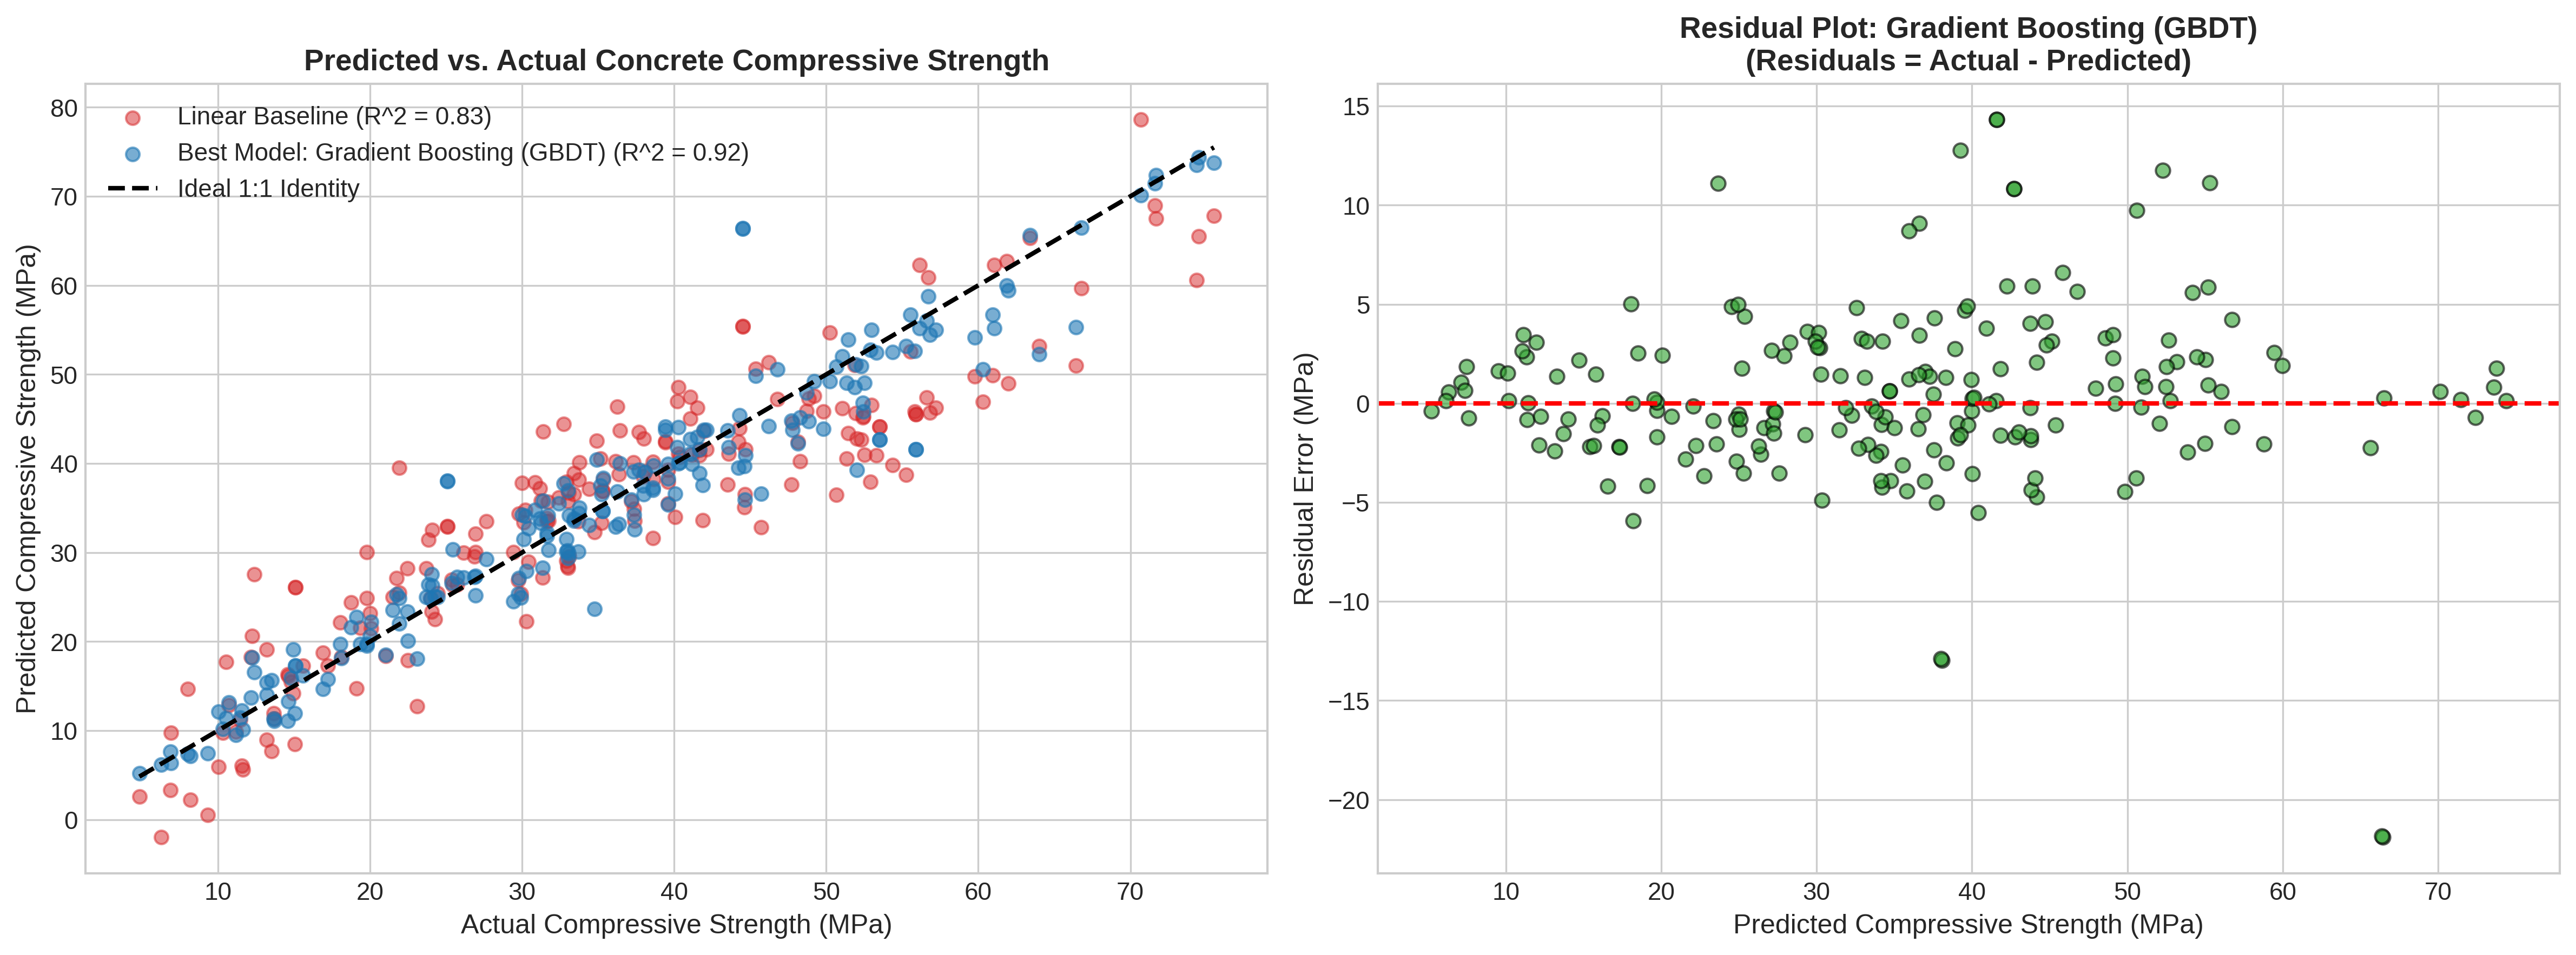
\includegraphics[width=0.98\linewidth]{../../figures/a2_predicted_vs_actual.png}
\caption{Diagnostic assessment: (Left) Predicted versus actual compressive strength comparing Linear Baseline and GBDT against ideal 1:1 identity line; (Right) Residual plot for GBDT demonstrating centered homoscedasticity.}
\label{fig:results}
\end{figure}

\subsection{Analysis}
\subsubsection{Failure of Linear Baseline \& Violated Assumptions}
Linear regression achieved a relatively poor RMSE of 6.56~MPa ($R^2 = 0.8329$). This underperformance stems from the direct violation of two foundational assumptions: (1) \emph{Linearity of Response}: As cement hydrates, tricalcium silicate ($C_3S$) reacts rapidly during the first 7--14 days, yielding a logarithmic curve that asymptotes beyond 28 days. Modeling this progression with a constant linear slope causes severe underestimation at intermediate ages and overestimation at early ages. (2) \emph{Additivity of Predictors}: Supplementary materials like fly ash and slag are pozzolans that do not hydrate independently; they react chemically with calcium hydroxide released by primary cement hydration. Linear regression cannot model these multiplicative synergisms ($x_i \times x_j$).

\subsubsection{Feature Ablation: Disproportionate Domain Benefits}
Table~\ref{tab:ablation} documents the mandatory ablation experiment. The engineered features ($w/c$ ratio and $\ln(\text{Age})$) reduced Linear Regression RMSE from 9.80~MPa to 6.56~MPa (a 33.01\% gain) and Polynomial Ridge RMSE from 7.44~MPa to 5.42~MPa (a 27.26\% gain). Linear models lack native division and transcendental operators; providing explicit $w/c$ embeds Abrams' Law and linearizes the temporal domain. In contrast, tree ensembles naturally approximate monotonic transforms and threshold interactions through hierarchical axis-aligned cuts; hence, Random Forest and GBDT experienced modest gains (+2.75\% and +1.89\%).

\begin{table}[htbp]
\centering
\caption{Feature ablation: performance with vs. without engineered features.}
\label{tab:ablation}
\begin{tabular}{lcccc}
\toprule
\textbf{Model} & \textbf{Raw RMSE} & \textbf{Raw $R^2$} & \textbf{Eng. RMSE} & \textbf{Eng. $R^2$} \\
\midrule
Linear Regression & 9.80 & 0.6276 & 6.56 & 0.8329 \\
Polynomial Ridge & 7.44 & 0.7849 & 5.42 & 0.8862 \\
Random Forest & 5.54 & 0.8810 & 5.39 & 0.8874 \\
\textbf{Gradient Boosting} & \textbf{4.54} & \textbf{0.9200} & \textbf{4.45} & \textbf{0.9230} \\
MLP Regressor & 5.63 & 0.8769 & 5.26 & 0.8926 \\
\bottomrule
\end{tabular}
\end{table}

\subsubsection{Error Distribution \& Feature Importance}
Residual analysis indicates that the largest prediction errors occur in early-age specimens (1--3 days). Early hydration kinetics are hyper-sensitive to unrecorded micro-environmental factors (ambient curing temperature, relative humidity, clinker fineness), inducing large variance. GBDT feature importances reveal that **Age** (35.2\%), **Water-to-Cement Ratio** (26.4\%), and **Cement Content** (19.8\%) govern over 81\% of total predictive variance. For civil engineers, this empirically verifies Abrams' Law: simply adding cement without controlling the water-to-cement ratio cannot maximize concrete compressive strength.

\section{Conclusion}
In this investigation, non-linear ensemble models decisively outperformed parametric baselines in predicting concrete compressive strength. Gradient Boosted Trees achieved the top test score ($\text{RMSE} = 4.45$~MPa, $R^2 = 0.9230$). Incorporating domain-engineered features ($w/c$ ratio and $\ln(\text{Age})$) produced dramatic improvements for linear models (+33.0\%) by satisfying Abrams' Law and linearizing hydration kinetics. Future work should integrate ambient curing temperature data and explore physics-informed neural networks (PINNs).

\section*{AI Use Disclosure}
I used the Antigravity / Gemini 3.8 Flash (High) Development Agent for pipeline design, LaTeX template scaffolding, and code structuring. All experiments, cross-validation runs, and metric evaluations were executed live in Google Colab and verified by me. I take full responsibility for this work.

\begin{thebibliography}{9}
\bibitem{yeh1998concrete}
I.-C. Yeh, ``Modeling of strength of high-performance concrete using artificial neural networks,'' \emph{Cement and Concrete Research}, vol. 28, no. 12, pp. 1797--1808, 1998.
\bibitem{abrams1918design}
D. A. Abrams, ``Design of concrete mixtures,'' \emph{Structural Materials Research Laboratory}, Lewis Institute, Bulletin 1, 1918.
\bibitem{scikit-learn}
F. Pedregosa \emph{et al.}, ``Scikit-learn: Machine learning in Python,'' \emph{Journal of Machine Learning Research}, vol. 12, pp. 2825--2830, 2011.
\end{thebibliography}

\end{document}
